Os resultados deste capítulo referem-se ao gráfico de preço, volume e transações do Bitcoin, em intervalos de 15 minutos, ao longo de nove meses em 2020 (GMT -3).
Foram utilizados dados da Binance para o par BTC/USDT, com uma implementação própria chamada BTools, cobrindo o período de 01/01/2020 a 01/10/2020, representando 271 dias e 26.304 entradas.
Esse conjunto de dados foi então armazenado em um arquivo CSV e posteriormente carregado em memória para o treinamento dos modelos supervisionados e ajuste dos modelos estatísticos.

\section{Validação de completude}
O \textit{Dataset} continha 59 valores duplicados que foram complementados por outros 59 entradas faltantes, aos quais foram removidos e preenchidos com o número anterior, respectivamente.
Tal fenômeno ocorreu provavelmente devido a manutenções e atualizações da Binance, visto que ao buscar o horário separadamente, a API retornava erro.

\section{Tratamento e pré processamento de dados}
Para o aprendizado supervisionado os dados foram escalonados utilizado o MinMaxScaller, conforme a equação \ref{eq:scalled}. Os conjuntos de treinto, teste e validação foram divididos de acordo com a tabela \ref{tab:conjuntos} em 60\%, 20\% e 20\% respectivamente. 
O janelamento utilizado foi de 24 entradas (6 horas) para prever o próximo valor de preço.

No ARIMA foi utilizado o método de auto arima para encontrar os melhores parâmetros p, d e q com base no primeiro janelamento (treino).

\begin{table}[!htb]
    \caption{Dados da divisão em conjuntos} \label{tab:conjuntos}
    \begin{tabularx}{\textwidth}{X|X|X|X|X}
    \hline
    Nome & Inicio & Fim & Horas & Entradas \\ \hline
    Treino   & 01/01/2020      & 25/02/2020            & 1315      & 5261          \\ \hline
    Teste   & 25/02/2020     & 20/04/2020            & 1315     & 5261         \\ \hline
    Validação   & 20/04/2020      & 01/10/2020             & 3945     & 15782         \\ \hline
    \end{tabularx}
    \fonte{Elaborado pelo autor, 2024.}
\end{table}

\section{Treinamento dos modelo}
Os modelos supervisionados foram treinados com limite de 500 épocas, limitadas por 30 épocas de paciência, com um \textit{batch size} de 32.
Para o \textit{learning rate} a taxa dinâmica foi implementada, com valor inicial de 0.001 e decaimento de 0.5 em platôs de 20 épocas.
A função de perda utilizada foi a Huber, que é menos sensível a \textit{outliers}.

O gráfico de convergência foi basicamente o mesmo para todos os modelos, com uma queda acentuada nas primeiras épocas, seguidas por leves degraus gerados pelo decaimento do \textit{learning rate}
e estabilização após 100 épocas, como mostra a figura \ref{figura:convergencia}.

\begin{figure}[!htb] \centering
    \caption{Gráfico de convergência} \label{figura:convergencia}
    \begin{varwidth}{\linewidth}
      \includegraphics[width=16cm]{figuras/convergência.png}
      \fonte{Elaborado pelo autor, 2024.}
    \end{varwidth}
  \end{figure}

O modelo ARIMA não pode ser treinado, mas, foi ajustado com os parâmetros (\textit{p} = 4, \textit{d} = 1 e \textit{q} = 5) através do conjunto de treino. Os conjuntos de teste e validação foram concatenados e a cada previsão o valor correto era inserido na janela.

\section{Visualização de resultados}
Esta seção apresenta os resultados dos modelos implementados neste estudo, seja através de gráficos ou detalhando os valores dos erros obtidos para cada abordagem. As métricas de erro foram calculadas para avaliar a precisão das previsões.

\subsection{\textit{Long Short-Term Memory}}

Os resultados do modelo LSTM são apresentados na Figura~\ref{figura:lstmOutput}, no qual é possível observar a previsão do modelo em relação ao preço real do Bitcoin. O modelo apresentou as seguintes métricas de erro: raiz do erro quadrático médio (RMSE) de 193.5493, coeficiente de determinação ($R^2$) de 0,8990 e erro percentual absoluto médio (MAPE) de 0,0145.

\begin{figure}[!htb] \centering
  \caption{Gráfico de preços reais e previstos - LSTM} \label{figura:lstmOutput}
  \begin{varwidth}{\linewidth}
    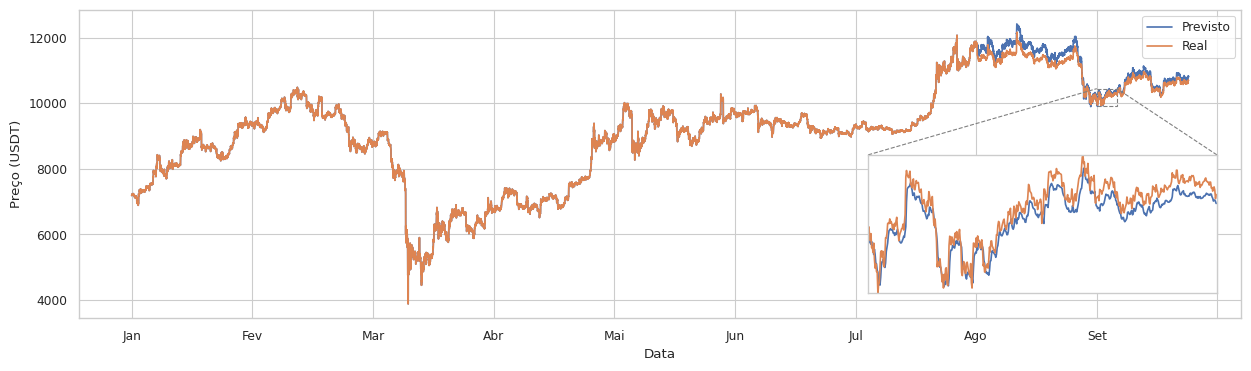
\includegraphics[width=16cm]{figuras/lstmOutput.png}
    \fonte{Elaborado pelo autor, 2024.}
  \end{varwidth}
\end{figure}



\subsection{\textit{Bidirectional Long Short-Term Memory}}

Os resultados do modelo BiLSTM são apresentados na Figura~\ref{figura:bilstmOutput}, no qual é possível observar a previsão do modelo em relação ao preço real do Bitcoin. O modelo apresentou as seguintes métricas de erro: raiz do erro quadrático médio (RMSE) de 207,2416, coeficiente de determinação ($R^2$) de 0,8842 e erro percentual absoluto médio (MAPE) de 0,0153.

\begin{figure}[!htb] \centering
  \caption{Gráfico de preços reais e previstos - BilSTM} \label{figura:bilstmOutput}
  \begin{varwidth}{\linewidth}
    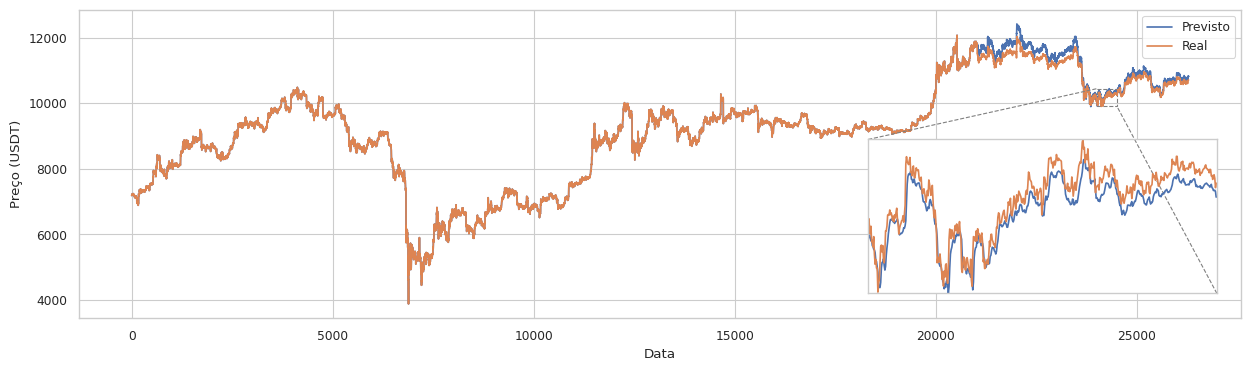
\includegraphics[width=16cm]{figuras/bilstmOutput.png}
    \fonte{Elaborado pelo autor, 2024.}
  \end{varwidth}
\end{figure}

\subsection{\textit{Gated Recurrent Unit}}

As previsões da arquitetura GRU são apresentados na figura \ref{figura:gruOutput}, dentre os modelos supervisionados implementados, este foi o que apresentou a menor raiz do erro quadrático médio (RMSE) de 86,1828, coeficiente de determinação ($R^2$) de 0,9799 e erro percentual absoluto médio (MAPE) de 0,0064.

\begin{figure}[!htb] \centering
  \caption{Gráfico de preços reais e previstos - GRU} \label{figura:gruOutput}
  \begin{varwidth}{\linewidth}
    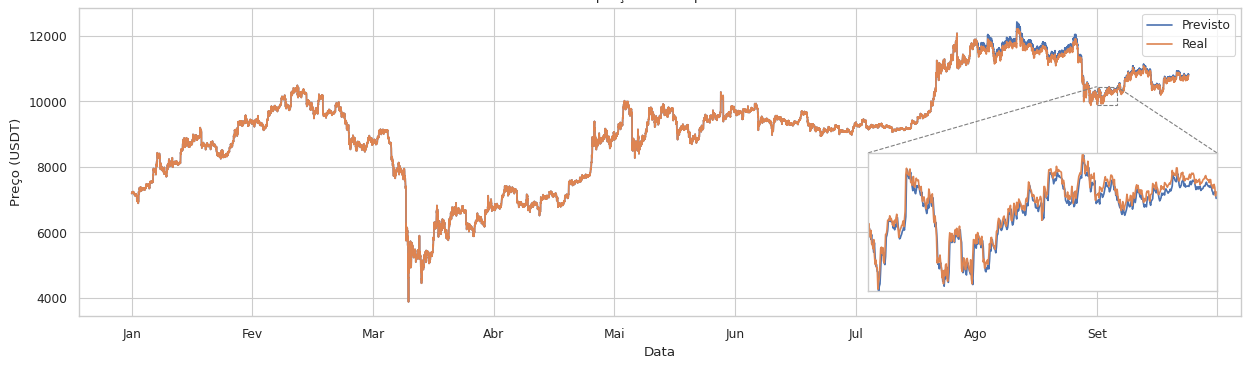
\includegraphics[width=16cm]{figuras/gruOutput.png}
    \fonte{Elaborado pelo autor, 2024.}
  \end{varwidth}
\end{figure}

\subsection{\textit{Auto Regressive Integrated Moving Average}}

Os resultados das previsões do ARIMA são apresentadas na figura \ref{figura:lstmOutput}, O modelo estatístico se destacou e apresentou a raiz do erro quadrático médio (RMSE) de 28,9699, coeficiente de determinação ($R^2$) de 0,9989 e erro percentual absoluto médio (MAPE) de 0,0016.

\begin{figure}[!htb] \centering
  \caption{Gráfico de preços reais e previstos - ARIMA} \label{figura:arimaOutput}
  \begin{varwidth}{\linewidth}
    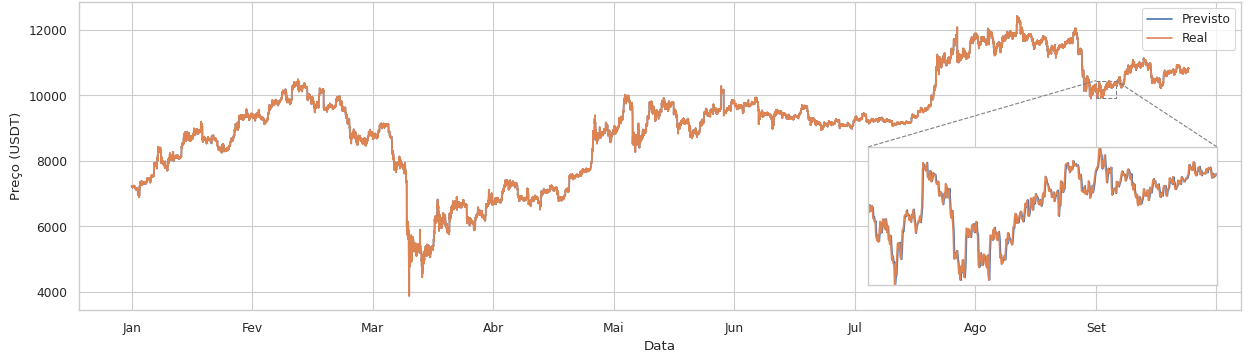
\includegraphics[width=16cm]{figuras/arimaOutput.png}
    \fonte{Elaborado pelo autor, 2024.}
  \end{varwidth}
\end{figure}

\section{Análise de resultados}

  A tabela \ref{tab:erros} apresenta os erros obtidos para cada modelo implementado neste estudo. O modelo ARIMA foi o que apresentou os melhores resultados, fato que pode estar ligado a natureza univariada e janelamento expansivo.
  No contexto dos modelos supervisionados, o GRU foi o que apresentou o melhor desempenho, seguido pelo LSTM e BiLSTM, respectivamente.
  A disparidade entre os modelos ressalta a complexidade do problema e a necessidade de mais estudos para aprimorar as previsões.
  Enquanto modelos estatísticos seguem uma abordagem mais simplista, os modelos de aprendizado profundo são mais complexos e podem ser explorados com outras \textit{Features} além de trocas e volume.

  No estudo em questão, foram exploradas diversas arquiteturas e hiperparâmetros nos modelos supervisionados, por isso, as taxas de erro foram mais baixas encontradas. 
  Mas, ainda há espaço para mais estudos, como a utilização de redes neurais convolucionais e redes neurais recorrentes com mecanismos de atenção, além de outras técnicas de processamento de linguagem natural e processamento de séries temporais.
  
\begin{table}[!htb]
  \caption{Erros em cada modelo} \label{tab:erros}
  \begin{tabularx}{\textwidth}{X|X|X|X|X|X}
  \hline
  Posição & Nome & RMSE & $R^2$ & MAPE \\ \hline
  1° & ARIMA   & 28,9699      & 0,9989           & 0,0016             \\ \hline
  2° & GRU   & 86,1828      & 0,9799             & 0,0064             \\ \hline
  3° & LSTM   & 193.5493      &  0,8990           & 0,0145                \\ \hline
  4° & BiLSTM   & 207,2416    & 0,8842            & 0,0153           \\ \hline
  \end{tabularx}
  \fonte{Elaborado pelo autor, 2024.}
\end{table}